%%%%%%%%%%%%%%%%%%%%%%%%%%%%%
\section{\syscrypt}
\label{s:eval-cryptdb}

We combine \sys with CryptDB to evaluate the cost of composing \sys's guarantees
with those of encrypted databases.
%
%To harden \sys's security guarantees, developers can deploy an \sys-enabled
%application atop an encrypted database such as CryptDB~\cite{cryptdb}.
%
CryptDB protects un\xxed database contents against attackers who compromise
the database server itself (with some limitations~\cite{grubbs}), in addition
to \sys's existing protections for \xxed data.
%
%We refer to the combination of \sys and CryptDB as \syscrypt.
%

%
%\textbf{Proxy Encryption and Decryption.}
\syscrypt operates in CryptDB's threat model 2 (database server and proxy can be
compromised).
%
A developer using \syscrypt deploys the application (and \sys) atop a proxy that
encrypts and decrypts database rows.
%
%\syscrypt operates on un\xxed data in the same way as CryptDB, and
%
% \syscrypt encrypts database rows with per-object keys; object keys are
% themselves
% encrypted with the public keys of the users who can access the object.
% %
% Only users who are actively using the application have their private keys in the
% proxy, so a proxy compromise only exposes the data these users have access to.
% %
% %
% On inserts or updates, \syscrypt generates keys for the new data, and encrypts
% the keys with the public key of users who own the data.
% %
% %Keys that are no longer needed are deleted from \fn{access\_keys}.
% %
% On reads, \syscrypt uses stored key-metadata to check if any accessible object key
% is associated with a retrieved object; if so, \sys decrypts the data with the
% key.
% %
% Like CryptDB, \syscrypt supports shared data by storing an encrypted copy of an
% object's key for each user who has access to the object.
%
%%
%The proxy stores encrypted object keys in an \fn{access\_keys} table mapping
%from user public key to their set of encrypted object keys.
%%
%The set of encrypted object keys is indexed by (both plaintext and encrypted)
%object identifiers, which allows for efficient lookup of object keys to encrypt
%or decrypt queries or query results.
%%
%
%\textbf{Developer Experience.}
%To use \syscrypt, application developers specify which users can
%access what data (\eg by specifying foreign keys that indicate ownership of
%objects).
%
%Developer-provided \xx specifications have this additional role in
%\syscrypt. \hmng{ this feels unclear. How do they do this? Just in the sense that it's
%implicitly already given in the schema description that Edna gets? }
%
Queries from \sys and the application operate unchanged atop the proxy, but to
ensure proper access to user data, the application and \sys must handle user
sessions.
%
\syscrypt exposes an API to log users in and out using their credentials.  Prior to applying
transformations to a user's data, \sys performs a login to ensure that \sys has
legitimate access to their data (\eg the user, an admin, or someone sharing the
data is logged in).

%
%Because the database is encrypted, \xxing transformations
%can only operate on data that logged-in users can access.

% and provide the proxy their private keys.
%with a couple of extra requirements to provide the proxy with private keys of
%logged-in users.
%
%
%Because the database is encrypted, \xxing transformations
%can only operate on data that logged-in users can access.
%
%\sys must also add an initial login before \xxing a user's data to ensure that
%\sys has legitimate access to their data (\eg the user, an admin, or someone
%sharing the data is logged in).
%
%, similar to how the application invokes \syscrypt with the user's private key
%to reveal data.
%

\syscrypt handles keys in the same way as CryptDB: \syscrypt encrypts database rows
with per-object keys, and object keys are themselves encrypted with the public keys
of the users who can access the object.
%
After a user logs in, the application gives the proxy their private key, thus
allowing decryption of their accessible objects.
%to the proxy, and can access only those
%objects encrypted with their public keys.
%\syscrypt handles keys in the same way as CryptDB, \ie encrypting objects with
%per-object keys, and granting users access via which object keys they own.
%
% A \fn{LOGIN} request includes the user's credentials, which \syscrypt uses to
% derive the user's private key and forward it to the proxy. The proxy uses the
% private key to decrypt the user's accessible object keys and access the
% plaintext object data.
% %
% %
% A \fn{LOGOUT} request tells the proxy to remove all decrypted object keys for
% the user (and thus renders the proxy unable to decrypt the user's data).
% %
% As long as objects for a user only get created while the user is logged in,
% \syscrypt can batch-encrypt the entire set of object keys for the user when
% they log out.
% %
% Creating objects for logged-out users is possible as long as the principal's
% public key is available, but comes at a performance cost: these objects require
% creating a separately-encrypted set of object keys, which will increase
% decryption cost on the user's next login.
%

%As an optimization, if \syscrypt generates a user's object keys only when the
%user is logged in, then \syscrypt has access to the entire set of the user's
%object keys in plaintext. This lets \syscrypt batch encrypt the entire set at
%once when the user logs out.
%%
%Otherwise, if \syscrypt must store encrypted object keys for a user while the
%user is logged out, then \syscrypt does not have access to the user's
%entire set of object keys. \syscrypt must encrypt each object key individually
%with the user's public key, and store a set of encrypted keys (instead of an
%encrypted set of keys).
%%
%Regardless of how keys are encrypted, \syscrypt defers key deletion from
%\fn{access\_keys} until the user logs out.
%\lyt{Too much detail?}

%
%\syscrypt internally uses this API to ensure that \xxing transformations that
%change user ownership (perform decorrelations) properly encrypt data for
%pseudoprincipals.
%

%
%\textbf{\Xxing and Revealing.}
%

%\syscrypt requires developers to ensure that their \xx specifications touch
%only data accessible to the user who invokes the \xxing transformation.
%
%In addition, if a user's records during \xxing or revealing include speaks-for
%records, \syscrypt logs in the pseudoprincipals with the private keys encoded in
%the speaks-for records.
%
%
%\syscrypt performs data removal and data modification identically to \sys, aside
%from the initial login of users. Decorrelation additionally ensures that
%encrypted decorrelated data can still be accessed by the original user.
%
%Decorrelation, however, requires slightly more nuance: for each new
%pseudoprincipal $p$ produced, \sys must ensure that a client speaking for $p$
%can access both $p$'s account object (\eg a \fn{users} table row) and
%the objects correlated to $p$. To do so, \sys encrypts (with $p$'s key) the
%keys associated with $p$'s account and any correlated objects.
%stores an
%encrypted copy of both the pseudoprincipal object's key and an encrypted copy of
%the recorrelated object's key, so that the pseudoprincipal can access both its
%account data and its now-owned object.
%
%\ms{I don't quite understand the last bit; let's discuss.} \hmng{ seconded. }
%

%\lyt{Could just get rid of this so we're not storing so many extra keys.}
%\syscrypt allows the decorrelated, original principal owning the object to
%store encrypted copies of the pseudoprincipal object's key and retain an
%encrypted copy of the recorrelated object's key. This leaks no additional
%information about which objects the original principal was correlated with,
%while allowing the original principal to access the object if logged in after
%decorrelation (\eg to edit after anonymization).

%\textbf{Limitations.}
%
%\syscrypt's key management imposes some limitations on applications that are
%absent in plain \sys.
%
%In particular, all
%

%\textbf{WebSubmit Evaluation.}
%We run WebSubmit on top of \syscrypt so that all WebSubmit answers and user
%accounts are always encrypted in the application database.  We also support
%account removal and answer anonymization using \syscrypt.
%%
%This required modifying WebSubmit to add API calls to \syscrypt to \fn{LOGIN}
%and \fn{LOGOUT} users when they signed in and out of their user accounts.
%%
%In addition, the developer specifies which users share what data. In the case of
%WebSubmit, the admin shares answers and user accounts with all existing users;
%all other users simply own their accounts and the answers they submit.
%%
%
%%
%Because users are always logged in when they add, edit, or read their data,
%\syscrypt can optimize encryption of user object keys in \fn{access\_keys}, and
%batch-encrypts each non-admin user's set of object keys. The admin's object keys
%are individually encrypted with the admin's public key, as the admin is not
%always logged in when user answers are submitted, or accounts created.
%%

%\textbf{Takeaways.}
%While \syscrypt provides stronger guarantees, it comes with both significant
%performance cost and the additional burden on the developer to properly manage
%user login and logout (although \syscrypt can support automatic, time-based
%logouts). In addition, \syscrypt's overheads will likely only grow for more
%complex applications, for which more complex encryption and key management
%schemes must be implemented (\eg to support joins over the data of multiple
%users). However, \syscrypt demonstrates that adding the guarantees of an
%encrypted database is not fundamentally at odds with \sys, and is in fact an
%orthogonal challenge.

%
%\textbf{Implementation.}
%
Our prototype only supports the CryptDB deterministic encryption scheme
(AES-CMC encryption), which limits it to equality comparison predicates. It also does not
support joins, a limitation shared with multi-principal CryptDB.
%
%Our implementation uses per-object keys that differ across tables, so
%it does not support \fn{JOIN}s, a limitation shared with multi-principal
%CryptDB (threat model 2).
%
%encrypts only sensitive object columns (\eg answer text and authors), leaving
%non-sensitive tables and columns, such as lectures, in plaintext.
%

\begin{figure}[t]
  \centering
      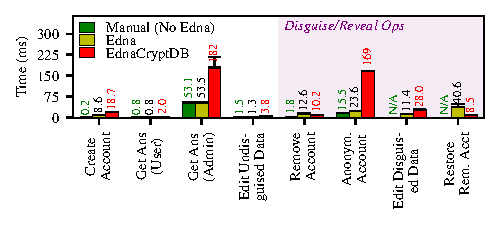
\includegraphics[width=\columnwidth]{figs/websubmit_cryptdb_op_stats}
    \caption{Latencies of WebSubmit (2k users, 80 answers/user) operations when
    implemented with \syscrypt (adding encrypted database support).
    Bars show median latency; error bars are
    5\textsuperscript{th}/95\textsuperscript{th} percentile latencies.}
  \label{f:cryptdb_ws_opstats}
\end{figure}

%
\textbf{Performance.}
We measure the latency of WebSubmit operations like before, and compare a manual
baseline, \sys, and \syscrypt.
%
\syscrypt is necessarily more expensive than \sys, and a good result for
\syscrypt would therefore show moderate overheads over \sys, and acceptable
absolute latencies.
%

%
Figure~\ref{f:cryptdb_ws_opstats} shows the results.
%
Normal application operations are 2--3$\times$ slower with \syscrypt than in
\sys, with the largest overheads on operations that access many rows, such as
the admin viewing all answers.
%
\Xxing and revealing operations are also 2--6$\times$ slower than \sys.
%

%
These overheads result from the cryptographic operations and additional
indirection in \syscrypt.
%
\syscrypt relies on a MySQL proxy, which adds latency: a no-op
version of our proxy makes operations 1.03-1.5$\times$ slower.
%proportional to the number of queries the operation issues.
%
%Further overheads come from object key management and computation necessary
%to properly encrypt query values or decrypt returned rows.
%
Cryptographic operations themselves are cheap ($<0.2$ms), but every object
inserted, updated, or read also requires lookups to find out which keys
to use, query rewriting to fetch the right encrypted rows, and
execution of more complex queries.
%

%
This is particularly expensive
when the user owns many keys (\eg the WebSubmit admin).
%
%\syscrypt maintains indexes that map object identifiers to keys for each
%user, but these indexes may not always determine which single key should be used.
%
%For example, a \fn{SELECT} query of the form \fn{SELECT * FROM answers WHERE
%email = 'some@email'} requires translating the value \fn{'some@email'}
%to ciphertexts that match all rows that encrypt answers with this email address.
%
%These rows use different keys, so after resolving the keys to use, \syscrypt
%issues a query of the form \fn{SELECT * FROM answers WHERE email IN
%(encrypted\_email1, encrypted\_email2, $\dots$)}.
%
%The index lookups to determine which keys to use and the increased query
%complexity add overhead, particularly when the user owns many keys (as in the
%case of the WebSubmit admin).
%
Admin-applied anonymization incurs the highest overhead (+143.6ms) as it issues
many queries to read user data and execute decorrelations.
%
Among the common operations,
an admin getting all the answers for a lecture
suffers similar overheads (+132.9ms).
%
%the admin possesses keys for all users's answers.
%Although \syscrypt indexes \fn{access\_keys} by object identifiers, queries that
%filter answers by partial object identifiers (\eg only lecture ID) will match
%against all keys of all users' answers, and thus require more encryptions to
%correctly apply queries.
%
%In contrast, individual users only have keys for their
%own answers, and thus often only perform one encryption (or decryption) per
%query (incurring a 2-5$\times$ overhead).

%%
%While non-trivial, these overheads may still be acceptable for practical web
%applications, as absolute latencies remain in the hundreds of milliseconds.
%%
%The latency of \xx/reveal operations, which typically run asynchronously, is
%also less critical than that of normal application operations.
%%
%
%%
%Finally, \syscrypt incurs fixed costs from \fn{LOGIN} and \fn{LOGOUT}
%operations, which prepare state in the proxy.
%%
%\fn{LOGIN} of a non-admin user takes a median of 10.2ms to decrypt and index the
%user's set of object keys;
%%: \syscrypt decrypts the user's set of object keys, and indexes each key by
%%object identifiers (\eg an answer's lecture and question IDs) for efficient key
%%lookups.
%%
%\fn{LOGOUT} of a non-admin user takes a median of 0.9ms to reencrypt the user's
%keys.
%%: \syscrypt updates, serializes, and encrypts the set of keys to store.
%%removes any keys to delete from the user's set of object keys; then
%%\hmng{When would the set of keys to be removed
%%not be all of them?}
%%
%Our \syscrypt prototype eagerly decrypts all keys for a user on login, causing
%expensive logins for users with lots of data (\eg 19s for the admin); this cost
%is not fundamental and \syscrypt could lazily decrypt keys when required.
%%, which would speed up login at the cost of additional per-query overhead.
%%

%\textbf{Security of \syscrypt.}
%
%\syscrypt combines CryptDB's protection of un\xxed data currently in the
%%database, with \sys's protection of \xxed data.
%%
%As \syscrypt executes vanilla \sys over an encrypted database, \syscrypt
%provides the same guarantees as \sys regarding confidentiality of the contents of
%\xxed data.
%%
%In addition, \syscrypt protects of the confidentiality of the contents of
%\emph{un\xxed} data in the application database against compromise of the
%database server, subject to the well-known limitations of encrypted
%databases~\cite{grubbs}.
%%
%An attacker sees only encrypted data, as every query goes through \syscrypt's
%proxy, and data stored/retrieved is encrypted/decrypted by the owning users'
%keys.
%%
%Like CryptDB, \syscrypt does not protect a user $u$'s un\xxed data if
%the attacker (1) compromises a user authorized to view $u$'s data (\eg an admin);
%or (2) compromises the application or proxy while $u$ is logged in.
%

%\textbf{\syscrypt.}
Like CryptDB, \syscrypt increases the database size (4--5$\times$ for our
WebSubmit prototype).
%
\syscrypt also stores an encrypted object key and its metadata (1KB per key) for
each user with access to that object.
